\documentclass[11pt]{article}

\usepackage{fullpage}
\usepackage[utf8]{inputenc}
\usepackage{graphicx}

\begin{document}

\title{ARM Checkpoint }
\author{Diego Cupello      (dc1020)\\
Norberto Mateos Camara     (nm920)\\
Andrey Popov               (ap4220)\\
Agustin Sotero Bourel      (as1920)\\}

\maketitle

\section{Group Organisation}

At first, we did not know well how to break down the tasks, since we still did not know well what to do for the emulator, as different group members were at different stages with the content of the lectures and the JMC people had not cover much of the computer architecture material. As such, we created a discord group and met to read the spec together, to clear up any doubts. \\ \\

After that, we divided ourselves roughly to work on different parts of the emulator. At first, two people were supposed to do handling the instructions and execution, while the others worked on the implementation of memory and pipeline and the binary loader. However, due to our poor coordination, there was some overlap in the work done, and a lot of changing in our implementation. One clear example of this was when we changed the memory implementation from 32-bit array to a 8-bit 2D array, and then later reverted it. This cost us some time which could have been avoided with better coordination and communication. \\ \\

Our group was able to work quite efficiently, and finished the emulator in a timely manner, despite the adequate coordination. We did meet up with our mentor, who advised to meet up periodically and create two git branches, instead of one, even if the project is small, in order to be able to split the later tasks in a better way. This will improve our coordination and also let us work more efficiently.

\section{Implementation Strategies}

We settled on implementing the ARM11 memory as a 32-bit word array, making it easy to put instructions inside the array and manipulate them. We created various utility functions that work with this implementation, and in the end it proved to be a good implementation, as it is easy to understand, and also quite easy to manipulate. There was one hard problem that came with this memory layout, which was loading and storing at address not multiples of four. Since it was 32-bit array we had to carefully store at specific bytes in two array accesses which proved to be quite challenging and not so clean. The pipeline was designed as a two entry array, the first slot containing the fetch instruction, and the second containing the decode instruction. Once its full, it takes the last element, executes it, and pushes once more to simulate the behavior of the pipeline. \\ \\

We structured the emulator in four main files: inhandler.c in instruction handler which contains all the functions necessary to check that instructions are a certain type as well as to check the state of the possible flags in the registers, utilities.c which handles shifting operations and useful functions such as getNBits and pushPipeline, execute.c, which handles the execution of instructions, and emulate.c which contains the main loop with the pipeline, and a function for printing the end state of the ARM machine to match that of the tests. We also have a testsuite.c, that provides test specific functions. The dependencies can be seen in this diagram:  \\

\begin{figure}[htp]
    \centering
    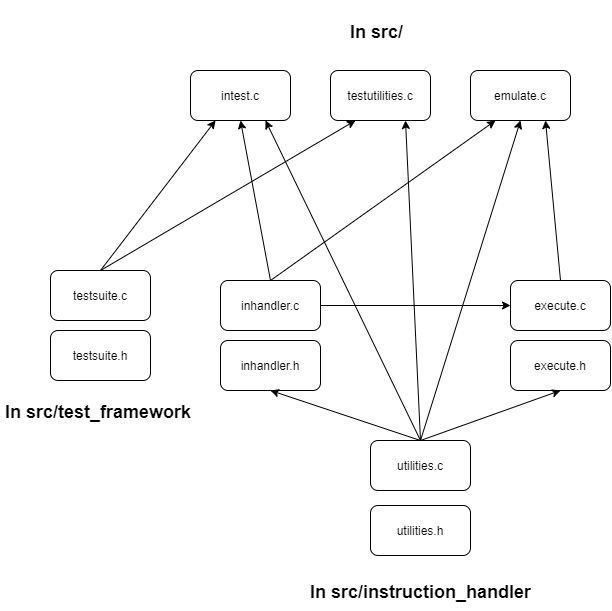
\includegraphics[width=8cm]{IncludesDiagram.png}
    \caption{Dependencies Diagram}
    \label{fig:files}
\end{figure}

Since the implementation of most functions were very specific, they will be hard to reuse. However there are some functions that we think we will be able to reuse. For example, we will use the functions in testsuite.c to create tests for the assemble part. As well as the little endian to big endian conversion function will be useful to convert between both conventions. We could also probably utilize the various shifting functions. \\

Finally, we believe that the tasks that we will find challenging, after doing the emulator, would be assembling single data transfer instructions, considering utilizing the same memory implementation for consistency, could bring some problems, and we are trying to plan strategically on tackling this problem. Another task that could be challenging could be parsing the instructions, since we are quite inexperienced in that topic. To mitigate this, we could possibly research a good way to parse assembly instructions (such as splitting it into tokens).

\end{document}